\section{Language games}
\label{sec:language-games}

The experiments that are executed using language games have a similar structure as the experiments in the previous chapters, since those provided the basis for the language games.
% SD: But there is an importnat difference that now we have two neural netweorks, the sender and the receiver.
% DK: TODO

The language games in this research have an asymmetric setup.
One agent, the sender is shown some information and needs to generate a message.
This message is received by the second agent, the receiver.
The receiver needs to parse this message and combine it with the same information that the sender was presented with.
The receiver then makes a prediction, which is compared to the ground truth.
The game is set up prosocial, which means that both agents receive the same loss based on the receiver's prediction.
All weights of the agents are adapted in the same way.

The vocabulary that the sender can draw from to produce a message is made up of initially arbitrary symbols.
The meaning of these symbols is created as soon as the sender uses them in one of the message, and the receiver is able to use it to solve the task successfully.
Over time, specific meanings are reinforced and a language emerges.
The number of possible words, namely the size of the vocabulary can be varied.
% SD: But possibly you would describe the language game setup already before on the background or method chapter. I would move all text there and make the language games description much more detailed, also giving examples. What is happening in terms of interaction? How is this modelled with the neural networks? It is important to emphasise this difference.
% DK: TODO

First, we will discuss \emph{discrimination games}, because they have the simplest setup.
% SD: What is this setup?
% DK: TODO
Furthermore, other language games that research this topic use a very similar setup.
In the next step, we will describe \emph{caption generators} that are set up as a language game.
Here, the sender describes the scene, while the receiver needs to generate a caption.
In the last step, we try to lose as much human bias as possible and the models are trained on just 'pointing' towards the target object, by again predicting its center coordinates.
% SD: Why are we not testing it on all 3 games?
% SD: Not sure what you mean here? Why do we loose human bias? 
% DK: TODO

The languages that emerge are analyzed in two ways.
An analysis of the frequency of used symbols and messages, as well as an examination for which images and objects they are used indicates the structure of the language and meanings of the symbols.
In a second step, the language is compared to several referring expressions in natural language.
By doing this, it can be seen if the models learned to use similar ways of referring to objects as humans do, or if they rely on different approaches.

\subsection{Object identification}
\subsubsection*{Setup}

In a discrimination game, the agents are presented with two or more images, one of these being the target image.
The sender needs to communicate this target image to the receiver by discriminating it from the other distractor images.
The receiver then needs to decide based on the message, which of the images is the target image.

The discrimination games in this research have a very similar setup as described in \citep{Lazaridou2017}.
The agents in this research resemble their \emph{agnostic sender} as well as their \emph{receiver}.
One central difference is the production of the message.
The main goal of their language game was the identification of the concept that and image was related to.
Therefore, the sender communicated only single-symbol messages to the receiver, which should describe the concept of the target image.
Opposed to that in this research, the agents are tasked to discriminate objects from each other based on their attributes.
% SD: On the contrary,...
% DK: TODO
It is therefore assumed that the sender will communicate these discriminative attributes.
For that reason, the sender is allowed to generate sequences as a message.

Both 'Dale' datasets are used to train the agents in this mode.
Similarly to the bounding box classifier, bounding boxes around each of the objects are extracted and fed to the game.
As in \citep{Lazaridou2017}, the sender receives the bounding box of the target object as the first image, while the rest of the bounding boxes are shuffled.
% SD: Here it does not receive a boundig box of an object as in Lazaridou. They use whole images, don't they?
% DK: TODO
The sender is assumed to learn which of the input images is the target images by this approach.
The receiver receives the images in completely shuffled order.

\begin{figure}[h]
    \centering
    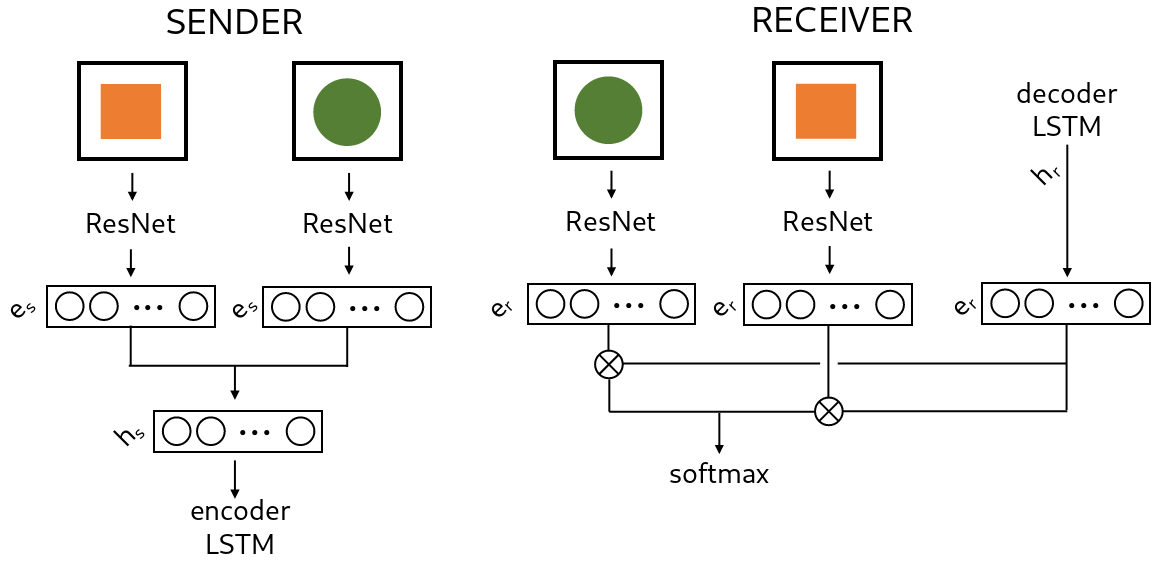
\includegraphics[width=.8\linewidth]{figures/arch_discriminator.png}
    \caption{Sender and receiver architectures in the discrimination game}
    \label{fig:discriminator_architecture}
\end{figure}

Figure \ref{fig:discriminator_architecture} shows, how the sender and the receiver of the discriminator are built up.
For the sender, the images are passed through a feature extractor and a following linear layer that reduces the dimensions to an embedding size $e_s$.
All embedded images are concatenated and passed through another linear layer to reduce the dimensions to the hidden size $h_s$.
This is then used as the initial state of the encoder LSTM in the sender wrapper.
% SD: Deatils about the layers, their parameters. More explanatory figure caption.
% DK: TODO

The receiver also encodes all images using a feature extractor with a following linear layer, reducing it to $e_r$.
The sequence, received by the sender is the input for its decoder LSTM, where the hidden state with a dimension of $h_r$ is randomly initialized.
As mentioned above, the receiver combines this image representation with the hidden state of each symbol separately.
This is done by passing the hidden state through a linear layer to scale its dimensions to the same $e_r$.
This allows the calculation of the dot product between it and the image representation.
If the message describes an object well, the resulting dot product should be higher.
The receiver then `points' to one of the images by applying the \emph{softmax} function over the results of the dot products.
The loss is calculated using the NLL-loss.

During the experiments, five variables are adjusted to compare their effects:
(1) the image embedding size for the sender $e_s$, (2) the LSTM hidden size for the sender wrapper $h_s$, (3) the image/message embedding size for the receiver $e_r$, (4) the LSTM hidden size for the receiver wrapper $h_r$ and (5) the size of the vocabulary $|V|$.

\subsection*{Results}
Table \ref{tab:results_discriminator} shows the accuracy of the models calculated on the success of communication if the receiver can identify the target object.
A random guess corresponds to 50\% in the \emph{Dale-2} dataset and 20\% in the \emph{Dale-5} dataset.
Four different vocabulary sizes $|V|$ are tested.
A size of 13 symbols corresponds to the 13 attributes the objects can have and align with human language.
If the symbols were similarly used, messages would have lengths between one and three symbols.
Opposed to that a slightly smaller vocabulary with 10 symbols is used to create a smaller bottleneck with a higher pressure to condense the information.
Similarly, a bigger vocabulary consisting of 20 symbols tests how a bigger bottleneck changes the results.
Lastly, a big vocabulary of 100 symbols should give the model all options to encode the information, including one symbol per attribute or one symbol describing a combination of attributes.
% SD: Motivation why this is so. The possible number of strings is {#colour} x {#shape} {object type} where all numbers except the last one also contain a padding token.
% DK: TODO

The hidden sizes $h_s$ and $h_r$ as well as the embedding sizes $e_s$ and $e_r$ are chosen in alignment with the vocabulary size.
The hidden sizes are always smaller or equal to the vocabulary size since the information about each word needs to be compressed in a smaller dimension to learn meaning.
Hereby, hidden sizes of 10 and 100 are tested.
On the other hand, three different embedding sizes are tested: 10, 50 and 100.
The reason for this is to experiment, what is the optimal middle ground between compressing features of an image encoded in high dimension vectors and upscaling encoded messages in low dimension vectors.
% SD: This discussion of dimensions could already be introduced when you discuss simple modles earlier as the same dimensions are used. This is a more an evaluation of represnetations rather than interaction and hence it would fit there.
% DK: TODO

\begin{table}[h]
    \centering
    \begin{tabular}{ccccc|cc|cc|cc}
        \toprule
              &         &         &         &         & \multicolumn{2}{c}{\textbf{Dale-2}} & \multicolumn{2}{c}{\textbf{Dale-5}} & \multicolumn{2}{c}{\textbf{CLEVR color}}                                                         \\\cmidrule(lr){6-7}\cmidrule(lr){8-9}\cmidrule(lr){10-11}
        $|V|$ & $h_{s}$ & $h_{r}$ & $e_{s}$ & $e_{r}$ & \textbf{Accuracy}                   & \textbf{length}                     & \textbf{Accuracy}                        & \textbf{length} & \textbf{Accuracy} & \textbf{length} \\\midrule
        {10}  & {10}    & {10}    & {10}    & {10}    & {96,4\%}                            & {0,99}                              & {24,7\%}                                 & {0}             & {17,3\%}          & {1}             \\
        {10}  & {50}    & {50}    & {50}    & {50}    & {50\%}                              & {1}                                 & {21,4\%}                                 & {1}             & {17,8\%}          & {0}             \\
        {13}  & {10}    & {10}    & {10}    & {10}    & {96,16\%}                           & {1}                                 & {24,8\%}                                 & {1}             & {17,1\%}          & {1}             \\
        {13}  & {10}    & {10}    & {50}    & {50}    & {49,6\%}                            & {1}                                 & {21,9\%}                                 & {1}             & {17,9\%}          & {0}             \\
        {20}  & {10}    & {10}    & {50}    & {50}    & {50,9\%}                            & {0}                                 & {23\%}                                   & {1}             & {15,9\%}          & {1}             \\
        {100} & {10}    & {10}    & {10}    & {10}    & {97,3\%}                            & {1}                                 & {24\%}                                   & {1}             & {18,1\%}          & {1}             \\
        {100} & {10}    & {10}    & {50}    & {50}    & {49,9\%}                            & {1}                                 & {24,4\%}                                 & {1}             & {15,8\%}          & {1}             \\
        {100} & {100}   & {100}   & {100}   & {100}   & {49\%}                              & {0}                                 & {25,3\%}                                 & {1}             & {15,6\%}          & {0}             \\
        \bottomrule
    \end{tabular}
    \caption{Results of the discriminators: $|V|$ are different vocabulary sizes, $h$ hidden sizes and $e$ embedding sizes.}
    % SD: A note about the datasets chosen. Why do we choose these? Initially, we describe more than 3 datasets.
    % DK: because the 'CLEVR Single' contains only one object. So there is nothing to discriminate (done)
    \label{tab:results_discriminator}
\end{table}
% SD: As we discussed at Semdial, it would be good to have a learning curves here that would show how fast or slow the languages converge. As David pointed out it may be that convergence is unstable and changes happen in between.
% DK: TODO

For the \emph{Dale-2}, a clear correlation between the hidden sizes, embedding sizes and the size of the vocabulary can be identified.
A hidden/embedding size as high as the vocabulary size is beneficial for identifying the correct object.
The receiver identifies almost every sample correctly when all sizes are 10.
When the hidden and embedding sizes are increased, the guesses by the receiver are random with 50\% accuracy.
Interestingly, a vocabulary size of 10 is enough to communicate a meaningful message when the model is trained on the \emph{Dale-2} dataset.
% SD: How do we know? What would happen if the hidden layers are smaller than the vocabulary size? We would also need to test several smaller dimensions.
% DK: because the task is solved succesfully, TODO

The results change, when using the \emph{Dale-5} dataset with four distractors.
With four distractors and with low hidden, embedding and vocabulary sizes, the agents barely pass the random baseline with 23\%.
Only increasing the vocabulary size to 100 raises the accuracy by almost 20\% points to 43\%.
This is still considerably lower than the 95\% of the \emph{Dale-2} dataset.
The same applies to the 'CLEVR color' dataset, where all models achieve a very low accuracy of around 15 to 17\%, corresponding to random guesses.
% SD: Could we say that calculation on Dale-5 is successful?
% DK: TODO

Two conclusions can be drawn.
First, the hidden as well as the embedding sizes need to be close to the vocabulary size.
% SD: Not sure, since we never tested smaller layer sizes. If the embedding layers are the same as the vocabulary size then at least a language encoding LSTM is not motivated to geenralise at all as it can keep representations for individual words without abstracting them. Leanring word embeddings involves reducing dimensions.
% DK: TODO
This even applies for very low vocabulary sizes, which means that the image encodings need to be compressed to the same low dimensions.
The reason for this is very likely that neural models have difficulties to upscale from lower dimensions (e.g. from low $h_r$ to high $e_r$) as opposed to learn how to extract the important information from a vector with many dimensions.
% SD: Hypothesis space to find the target function is just too big and they can never approximate that function.
% DK: TODO

The second conclusion that can be drawn looks at the differences between the two datasets.
Unsurprisingly, the agents have a much higher difficulty to discriminate a target object from four instead of one distractor.
Since we discriminate objects based on properties that are also distinguished in human cognition (8 colors, 2 sizes, 3 shapes), we expect that the vocabulary onto which the agents converge reflects these categories and is therefore close to human vocabulary.
There are $8*2*3=48$ possible combinations of attributes.
% SD: Calculation behind this figure?
% DK: (done)
Still, for Dale-2, a vocabulary size of only 10 is enough for an almost perfect accuracy with two objects.
This hints to the fact that the agents don't describe the complete target object, but only rely on discriminative attributes between the objects.
The need for a more detailed description of discriminative attributes is higher when more distractors are involved.
Therefore, the models need to learn more combinations of symbols in order to attest to this higher level of detail and especially how to relate them to features in the images.
% SD: We would need to show that the messages in Dale-2 are shorter than in Dale-5 to claim this.
% DK: TODO

\cmtDK{similarity to bounding box classifier}

\subsection{Referring expression generation}
\subsubsection*{Setup}

In a next step, it is tested if the agents can learn to extract features of the objects together.
For this, the receiver is tasked to describe the target object in natural language, while the sender needs to communicate, which object is the target.
Again, the setup is asymmetrical: the sender receives the image and information, which of the objects in the image is the target object in form of a masked image.
The receiver only sees the image without additional information.
\cmtDK{human bias vs emergent language}

This setup is based on the single neural model described above.
The target caption for each image is created using the GRE-algorithm of \citet{Dale1995}.
% SD: The sender uses the incremental algorithm?
% DK: TODO, QUESTION
Since the results of the experiments show that the position of the padding doesn't have an effect on the final converging scores, the padding tokens are only prepended to the caption.

\begin{figure}[h]
    \centering
    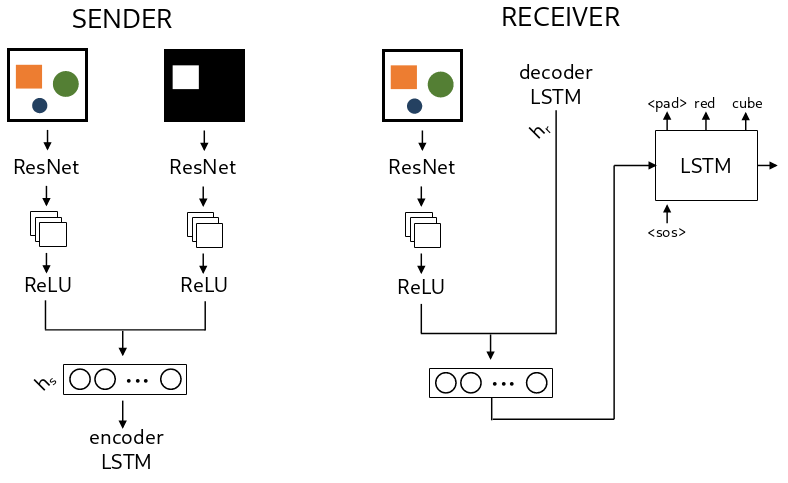
\includegraphics[width=.7\linewidth]{figures/arch_caption_generator_game.png}
    \caption{Simplified architecture of the caption generator game}
    \label{fig:caption_generator_game_architecture}
    % SD: But here we don't need an LSTM, we just want to identify one of the objects. The LSTM should only encode the inout message.
    % DK: TODO
\end{figure}

The sender is built up of two image encoders, one encodes the original target image and one encodes the masked image.
The image encoders are set up as described in \citep{Johnson2017}.
A feature extractor extracts basic features of the images.
Two following convolutional layers with a \emph{ReLU} function are trained to condense the most important information from the resulting matrices.
A max pooling layer and a linear layer reduce the dimensions to 1024 dimensions.
This size was found to have the best results during the experiments.
% SD: Reference back to when you reported this?
% DK: TODO
The two resulting encoded images are flattened and concatenated.
A final linear layer reduces this long vector to the hidden size of the message LSTM $h_s$, which is used as the initial hidden state of this LSTM.

The receiver uses the same architecture to encode the original image as the sender.
The resulting flattened vector is concatenated with the decoded message of hidden size $h_r$.
This is then passed through a linear layer, again reducing it to 1024 dimensions and is then used as the initial state of the captioning LSTM.
% SD: But receiver is not doing captioning? Is it incrementally identifying the objects as the sender's messages are coming in?
% DK: TODO
During training, the ground truth caption is used as the input to the LSTM using teacher forcing.
% SD: I'm not sure how teacher forcing is implemented, see my earlier comment
% DK: typo, teacher forcing is actually applied (done)
When presented with test data, the LSTM always produces three tokens, by using its own predicted words as the input for the next step.
The loss is calculated with cross entropy.

Since the agents are trained to describe the target object discriminatively based on the described GRE-algorithm, they are trained on the 'Dale-2' and 'Dale-5' dataset.
The 'Dale-5' should be again much harder to learn, since there are more objects that the agents need to discriminate the target object from.
% SD: So the sender is generating descriptions following the GRE policy?
% DK: TODO

During the experiments, the following variables are adjusted, and the results are compared:
(1) the vocabulary size $|V|$,
(2) the LSTM hidden size of the sender wrapper $h_s$ and
(3) the LSTM hidden size of the receiver wrapper $h_r$.
The same metrics as in the pre-experiments are used to evaluate the results.

\subsubsection*{Results}
\begin{table}[h]
    \centering
    \begin{tabular}{ccc|ccc|ccc}
        \toprule
              &         &         & \multicolumn{3}{c}{\textbf{Dale-2}} & \multicolumn{3}{c}{\textbf{Dale-5}}                                                                             \\\cmidrule(lr){4-6}\cmidrule(lr){7-9}
        $|V|$ & $h_{s}$ & $h_{r}$ & \textbf{Acc.}                       & \textbf{word-by-word}               & \textbf{length} & \textbf{Acc.} & \textbf{word-by-word} & \textbf{length} \\\midrule
        {10}  & {10}    & {10}    & {22,9\%}                            & {62,8\%}                            & {1}             & {7,1\%}       & {40\%}                & {1}             \\
        {13}  & {10}    & {10}    & {22,8\%}                            & {62,9\%}                            & {0}             & {7,3\%}       & {38,7\%}              & {1}             \\
        {20}  & {10}    & {10}    & {24,6\%}                            & {64\%}                              & {1}             & {6,7\%}       & {38,7\%}              & {1}             \\
        {100} & {10}    & {10}    & {24,4\%}                            & {62\%}                              & {1}             & {7,8\%}       & {40\%}                & {1}             \\
        {100} & {100}   & {100}   & {21\%}                              & {62\%}                              & {1}             & {6,5\%}       & {37,8\%}              & {1}             \\
        \bottomrule
    \end{tabular}
    \caption{Results of the caption generator: $|V|$ are different vocabulary sizes and $h$ hidden sizes.}
    % SD: What is word-by-word?
    % DK: the same as in the caption generator with a single model (QUESTION)
    \label{tab:results_caption_generator_game}
\end{table}

The results of the caption generator game are summarized in Table \ref{tab:results_caption_generator_game}.
In general, it can be seen that the agents have much bigger problems, to solve the task together than a single neural network.
The highest accuracy for descriptions, the agents manage to predict correctly is at 24,6\% for images of the 'Dale-2' dataset.
Compared to the (masked) accuracy of the single model with 72\%, the agents predict 47,4\% points less correct descriptions.
A similar worse performance can be seen for the 'Dale-5' dataset.
Here, the agents only manage to produce for 7,8\% of the images correct descriptions with a vocabulary size of 100, 13,2\% points less than the single neural model.
The same effect can be seen for the word-by-word accuracy, which is much lower than the metric for the single neural model for both datasets.
% SD: With the vocabulary size of 100.
% DK: (done)

When looking, how the different variables affect the performance, it can be seen that a bigger vocabulary size tends to help the agents.
% SD: Not sure. The difference is still very small, within a couple of %.
% DK: TODO
This is only visible for the 'Dale-2' dataset.
With constant hidden sizes of 10, the agents score around 22,9\% with only 10 and 13 available symbols.
When this is increased to 20 and respectively 100 symbols, the agents can increase their accuracy to around 24,5\%.
However, the increase is relatively small.
Interestingly, this effect only occurs, when the hidden sizes are small with only 10 dimensions.
As soon as they are increased to 100 dimensions with a vocabulary size of 100 symbols, the accuracy drops to 21\%.
% SD: Very small decerase for such a large difference in vocabulary size compared to what we have seen earlier.
% DK: TODO

Looking at the 'Dale-5' dataset, the increase is still there, when the vocabulary is increased to 100 symbols.
Nonetheless, the difference is with 0,5\% points even smaller and the reason may be due to other influences, such as the random initialization of the weights of the agents.
This is confirmed, when looking at emerged languages.
In all the setups, the same message is communicated for all samples, independently of the input image.
This is also reflected in the length of the messages.
For the setup with a vocabulary size of $|V| = 13$, no message is transferred, and the accuracy stays the same as in the other setups.
% SD: Here it would be much better to have a loss curve to show differences in loss between the number of communication events, the same could also be done for accuracy. Then we would have a clearer picture of how vocabulary size affects learning. It could be that with 100 vocabulary there is actually a better performance than before the final cut-off point. Is this possible? How was the final cut-off point determined anyway?
% DK: TODO

These results show that the agents are not at all able to encode meaning about the images and target objects in their messages.
% SD: Negative result: how can we then interpret that? What could we change? What did we learn from this?
% DK: TODO
This is especially interesting, compared to single model caption generator in section \ref{sec:referring_expression_generation}.
In these experiments, the model was able to converge towards correct captions and therefore able to extract the necessary information.
This shows that a main challenge for the agents lies in grounding symbols in these extracted features.

\subsection{Reference resolution}
\subsubsection*{Setup}
% SD: But previously we have said that we are not going to study this game. But good that we have!
% DK: where? (QUESTION)
In the final experiments, it is tried to eliminate as much human knowledge as possible.
% SD: Not true: human knowledge is still reflected in the way the environment is structured.
% DK: TODO
For that reason, the agents are tasked to only predict the location of the target object.
This task is approached in two steps.
In the first step the sender is still shown human knowledge in form of a description of the target object, since the previous experiments showed that the models were able to relate them to their own extracted features.
% SD: I'm not following this
% DK: TODO
The receiver doesn't come in contact with any human knowledge, not as input nor as output.
This approach acts as a sanity check if the agents are able to converge together on the correct target object coordinates.
In the second step, the caption is also removed from the sender.
Instead, a masked image points the sender towards the target object.
In this setup, no human knowledge is explicitly present, that can bias the emerged language to form similarly to human language, except for the implicit information in the image itself.
% SD: Which contains human knowledge!
% DK: TODO
With this, it can be analyzed, how the language between the agents emerges and which features or patterns are represented with symbols.

The agents are both set up in the same way as the single neural model, predicting the target object's coordinates.
The sender encodes the original image the same as in the previous paragraph.
In the first setup, the description of the target object is encoded, using an LSTM.
For this, an embedding with $emb_{descr}$ dimensions is learned to represent each word.
These embeddings are the input for the LSTM.
The final hidden state of $LSTM_{descr}$ dimensions is used as the representation of the whole description.
The vocabulary that is used for the descriptions is based on 14 symbols, including the padding token.
For the LSTM to learn a representation of each token as well as of the complete description, both $emb_{descr}$ and $LSTM_{descr}$ need to be smaller than the size of this vocabulary.
Choosing a size of 10 for both variables proved to give good results in the experiments.
In a next step, the image encoding and the final hidden state of the description are concatenated and passed through a linear layer to reduce the dimension to the hidden size $h_s$.
The resulting vector is passed to the sender wrapper LSTM, to generate the message.
% SD: Just thinking: would there be a more systematic way to compare all the models? Perhaps if you write the parameters in a table or a text that is parallel. Then you could simply say, modal A + these changes. It would be much clearer to the reader how all models are rerlated and it would be easier for the reader to follow.
% DK: TODO

\begin{figure}[h]
    \centering
    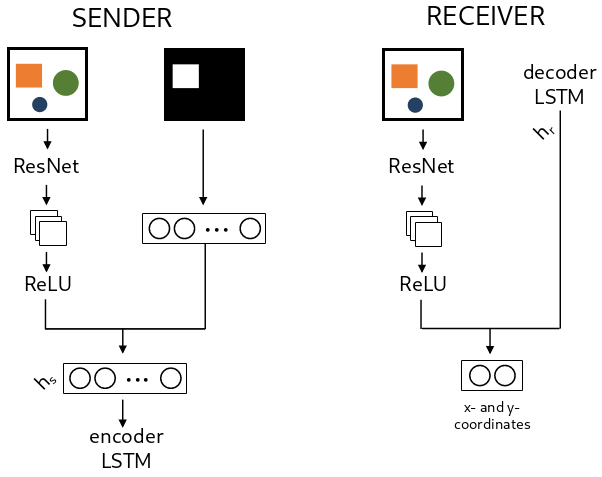
\includegraphics[width=.7\linewidth]{figures/arch_coordinate_predictor_game.png}
    \caption{Simplified architecture of the masked coordinate predictor game}
    \label{fig:coordinate_predictor_game_architecture}
    % SD: Again, why LSTM, are we inceremtally identifying the image while we are processing each input word?
    % DK: because it's a message sequence of discrete symbols (done)
\end{figure}

For the second approach, the masked image is passed only through a feature extractor.
Both the resulting encoding of the masked image and the encoding of the original image are each passed through separate linear layer to adjust their dimensions to the same embedding size $e_s$.
These embeddings are subsequently concatenated and reduced to the hidden size $h_s$ with a final linear layer.

The receiver contains of two parts.
First, the original image is encoded with an image encode of the same setup.
This encoded image is flattened and concatenated with the final hidden state of the wrapper LSTM encoding the message received by the receiver.
The resulting vector is the passed through the second part of the receiver, the predictor.
This predictor contains of three linear layers, reducing the dimensions to 1024, 1024 and 2 respectively.
A \emph{ReLU} function is applied in between.
This setup is trained to combine the important information from both the image and the message of the sender.
The euclidean distance between the resulting prediction of the center point and the true center of the target object is calculated and the weights of both agents are adapted accordingly.

As in the pre-experiments, the agents are trained first the 'CLEVR single' dataset to understand if they are capable of predicting locations in an image together.
In a next step, the 'Dale-2' and 'Dale-5' datasets are used to test if the agents are able to first communicate a target object and second describe the target object discriminatively with a small vocabulary.

During the experiments, the effects of the following variables are compared:
(1) the vocabulary size $|V|$,
(2) the LSTM hidden size of the sender wrapper $h_s$,
(3) the LSTM hidden size of the receiver wrapper $h_r$ and
(4) the embedding size of the sender $e_s$.
As before, the metrics to evaluate the results are the same as in the pre-experiments.

\subsection*{Results}
In the final setup, the agents are tasked with communicating objects with fewer infused human knowledge.
Table \ref{tab:results_dale_predictor_game} shows the results for the setup, in which the sender is pointed towards the target object with a human description based on the GRE algorithm.
Hereby, the 'CLEVR single' dataset acts as a baseline, to test if the agents are able to predict coordinates of objects at all.
In every configuration of the variables, the agents achieve a very high performance.
The worst average distance across the test dataset is 10 pixels, which still points onto an object.
Also the accuracy, which evaluates how many guesses of the receiver were pointing onto an object reflects this fact.
All configuration achieve an accuracy higher than 96,7\%.
% SD: Just occured to me: how do we measure accuracy if we are predicting numbers (numeric prediction)?
% DK: same as in the experiments with one model (done)
This aligns also with the results from the single neural models, where the average distance was similarly low.
In general, this shows that the agents are able to predict coordinates together.
However, the question arises if the message by the sender has actually an effect on the receivers' decision, or if the receiver learns to point towards the target coordinates on his own and the message is ignored.
Having a look at the transferred messages, it in fact shows that the receiver learns to point towards the target object on its own.
% SD: But how could it do so if the visual data is randomly distribution. It must rely on the message as that is the only source of information.
% DK: it does it in the same way as the single model above (TODO)
As in the experiment before, all communicated messages contain the same symbol independent of the input image.

\begin{table}[h]
    \centering
    \begin{tabular}{ccc|ccc|ccc|ccc}
        \toprule
              &         &         & \multicolumn{3}{c}{\textbf{CLEVR single}} & \multicolumn{3}{c}{\textbf{Dale-2}} & \multicolumn{3}{c}{\textbf{Dale-5}}                                                                                                       \\\cmidrule(lr){4-6}\cmidrule(lr){7-9}\cmidrule(lr){10-12}
        $|V|$ & $h_{s}$ & $h_{r}$ & \textbf{Dist.}                            & \textbf{Acc.}                       & \textbf{length}                     & \textbf{Dist.} & \textbf{Acc.} & \textbf{length} & \textbf{Dist.} & \textbf{Acc.} & \textbf{length} \\\midrule
        {10}  & {10}    & {10}    & {10,1}                                    & {98,5\%}                            & {1}                                 & {36,5}         & {19,9\%}      & {1}             & {45,7}         & {14,4\%}      & {1}             \\
        {13}  & {10}    & {10}    & {6}                                       & {99\%}                              & {0}                                 & {38}           & {20,4\%}      & {1}             & {47,3}         & {10,8\%}      & {1}             \\
        {20}  & {10}    & {10}    & {9,7}                                     & {96,7\%}                            & {1}                                 & {37,3}         & {21,2\%}      & {1}             & {47,3}         & {11,3\%}      & {0}             \\
        {100} & {10}    & {10}    & {7,7}                                     & {98,4\%}                            & {1}                                 & {40,4}         & {21,7\%}      & {1}             & {45,4}         & {10,8\%}      & {1}             \\
        {100} & {100}   & {100}   & {7,5}                                     & {96,9\%}                            & {1}                                 & {40,1}         & {17,8\%}      & {1}             & {44,3}         & {11,8\%}      & {0}             \\
        \bottomrule
    \end{tabular}
    \caption{Results of the description coordinate predictor: $|V|$ are different vocabulary sizes and $h$ hidden sizes.}
    \label{tab:results_dale_predictor_game}
\end{table}

When the experiments are run on the 'Dale-2' dataset, the results are much worse.
For the \emph{description coordinate predictor}, the average distance ranges from 36,5 pixels to 40,4 pixels.
The configuration with a vocabulary size of only 10 symbols fares the best, while a vocabulary of 100 symbols produces the worst results.
% SD: Remind the reader what is the size of the image so that they can interprert the distance relatively to that.
% DK: TODO
Still, the accuracy shows that around 19,9\% to 21,7\% of the guesses are on the target object.
Here, the configurations with higher vocabulary sizes fare slightly better, but the differences are very small and likely due to other factors.

The results for 'Dale-5' dataset are even worse, but are comparable with the results with a single neural model.
Apparently, the agents are not able to communicate the target object, and the predictions by the receiver are general in the middle of the image, which results in an average distance of around 45 to 50 pixels.
The differences of the mean distances are not very significant in this range, to allow an analysis of the different configurations.
% SD: I don't understand this
% DK: TODO

\begin{table}[h]
    \centering
    \begin{tabular}{cccc|ccc|ccc|ccc}
        \toprule
              &         &         &         & \multicolumn{3}{c}{\textbf{CLEVR single}} & \multicolumn{3}{c}{\textbf{Dale-2}} & \multicolumn{3}{c}{\textbf{Dale-5}}                                                                                                       \\\cmidrule(lr){5-7}\cmidrule(lr){8-10}\cmidrule(lr){11-13}
        $|V|$ & $h_{s}$ & $h_{r}$ & $e_{s}$ & \textbf{Dist.}                            & \textbf{Acc.}                       & \textbf{length}                     & \textbf{Dist.} & \textbf{Acc.} & \textbf{length} & \textbf{Dist.} & \textbf{Acc.} & \textbf{length} \\\midrule
        {10}  & {10}    & {10}    & {1024}  & {10,8}                                    & {93,1\%}                            & {1}                                 & {34,8}         & {24,3\%}      & {0}             & {44,3}         & {11,8\%}      & {1}             \\
        {10}  & {10}    & {10}    & {512}   & {9,3}                                     & {92\%}                              & {1}                                 & {36,3}         & {19,9\%}      & {0,7}           & {45,9}         & {12,7\%}      & {1}             \\
        {13}  & {10}    & {10}    & {1024}  & {7,8}                                     & {96,8\%}                            & {1}                                 & {36,3}         & {20,2\%}      & {0}             & {45,4}         & {11,4\%}      & {1}             \\
        {20}  & {10}    & {10}    & {1024}  & {6,6}                                     & {98,3\%}                            & {1}                                 & {37,8}         & {16,1\%}      & {1}             & {45,2}         & {11\%}        & {1}             \\
        {100} & {10}    & {10}    & {1024}  & {5,2}                                     & {98,5\%}                            & {1}                                 & {37,4}         & {20,1\%}      & {1}             & {43,6}         & {16,7\%}      & {1}             \\
        {100} & {100}   & {100}   & {1024}  & {12,5}                                    & {92,1\%}                            & {1}                                 & {36,5}         & {20,7\%}      & {1}             & {44,6}         & {12,7\%}      & {1}             \\
        \bottomrule
    \end{tabular}
    \caption{Results of the masked coordinate predictor: $|V|$ are different vocabulary sizes, $h$ hidden sizes and $e$ embedding sizes.}
    \label{tab:results_masked_predictor_game}
\end{table}

Finally looking at the setup, when using the masked image as an input shows that the results are similarly bad as when using the encoded captions.
This is easily explainable with the emerged language.
For both the experiments using the encoded captions and the experiments using masked images as input, no meaningful symbols are transferred.
% SD: A bit gloomy result. Negative result is okay but then we need an explanation why this is so and have some ideas what to change. What we can learn from these results?
% DK: TODO
Following, the receiver needs to solve the task alone and the different setups of the sender don't play any role in the overall success.
% SD: This identifies that the problem lies in how the sender encodes the messages; what is its policy to generate longer strings or reuse the word. Without a policy the sender will never be motivated to encode longer messages and therefore rely on single-word expressions.
% SD: The second problem is the size of these networks. We should also test smaller embedding sizes than 10. Practice shows that the embedding sizes can be even several magnitues smaller than the vocabulary sizes, cf. the Bengio paper and word2vec.
% SD: The reason why the system is not performing well on the pointing task is that it does not have the right features to learn from. It ahs visual information WHAT these objects are (what do they look like) but they do not have information WHERE these objects are,. John Kelleher and I wrote an opiiuon piece about the lack of spatial knowledge required to model spatial descriptions in CNNs. The same problem is probably occuring here. Replacing the features or adding geometric features that would communicate geometric relations that allow pointing would improve the task and also we would expect that a vocabulary would emerge such that some words are more biased towards visual features (to identify objects) and some more to geometric features (to locate them), hence WHAT and WHERE.
% SD: J. D. Kelleher and S. Dobnik. What is not where: the challenge of integrating spatial representations into deep learning architectures. In S. Dobnik and S. Lappin, editors, Proceedings of the Conference on Logic and Machine Learning in Natural Language (LaML 2017), Gothenburg, 12 –13 June, volume 1 of CLASP Papers in Computational Linguistics, pages 41–52, Gothenburg, Sweden, November 2017. Department of Philosophy, Linguistics and Theory of Science (FLOV), University of Gothenburg, CLASP, Centre for Language and Studies in Probability.https://gup.ub.gu.se/publication/262970?lang=en
% SD: Overall, the thesis has a lot of potential if we could implement all this
% DK: TODO

When comparing these results to the neural models in Section \ref{sec:reference_resolution} that are not part of a language game, it can be seen that the metrics are very similar for all datasets.
The model was already not able to solve the task without the increased complexity of a language game.
This therefore indicates that the challenge for the agents doesn't lie in grounding the extracted features in new symbols, but already in extracting the features in the first place.